%!TEX root = ../thesis.tex
% ******************************* Thesis Appendix B ********************************

\chapter{Analytic computation of eigenvalues for zonal functions}
\label{app:sec:compute-eigenvalues}


The eigenvalues of a zonal function are given by the one-dimensional integral:
\begin{equation}
    \label{appendix:theorem:funk2}
    \lambda_{n} = 
   \frac{\omega_{d}}{C_n^{(\alpha)}(1)} \int_{-1}^1 s(t)\,C_n^{(\alpha)}(t)\,(1 - t^2)^{\frac{d-3}{2}} \calcd{t},
\end{equation}
where $C_n^{(\alpha)}(\cdot)$ is the Gegenbauer polynomial of degree $n$ with $\alpha = \frac{d-2}{2}$ and $\omega_{d} = \Omega_{d-2} / \Omega_{d-1}$ denotes the surface area of $\dsphere$ (see \cref{app:sec:harmonics} for analytical expressions of these quantities). The shape function $s(t)$ determines whether this integral can be computed in closed-form. In the next sections we derive analytical expressions for the eigenvalues of the Arc Cosine kernel and ReLU activation function in the case the $d$ is odd. For $d$ even, other kernels (e.g., Mat\'ern) or activation functions (e.g., Softplus, Swish, etc.) we rely on numerical integration (e.g., Gaussian quadrature) to obtain these coefficients. We will show that both approaches lead to highly similar results.

\subsection{Arc Cosine kernel}
\label{sec:appendix:compute-eigenvalues-arccosine}

The shape function of the first-order Arc Cosine kernel \citep{cho2009kernel} is given by:
\begin{equation}
    s:[0, \pi] \rightarrow \Reals,\quad s: x \mapsto \sin x + (\pi - x) \cos x,
\end{equation}
where we expressed the shape function as a function of the angle between the two inputs, rather than the cosine of the angle. For notational simplicity, we also omitted the factor $1 / \pi$.

Using a change of variables we rewrite \cref{appendix:theorem:funk2}
\begin{equation}
    \lambda_n
    =  \frac{\omega_{d}}{C_n^{(\alpha)}(1)}  \int_{0}^\pi s(x)\,C_n^{(\alpha)}(\cos x) \sin^{d-2} x\,\calcd{x},
\end{equation}
% with $c_{d, n} = \frac{\omega_{d-2}}{C_n^{(\alpha)}(1)}$.

Substituting $C_n^{(\alpha)}(\cos x)$ by its polynomial expansion (\cref{appendix:eq:gegenbauer}), it becomes evident that we need a general solution of the integral for $n,\,m \in \Naturals$
\begin{equation}
\int_0^\pi \left[ \sin(x) + (\pi - x) \cos(x) \right] \cos^n(x) \sin^m(x) \calcd{x}.
\end{equation}

The first term can be computed with this well-known result:
% \footnote{\url{https://math.stackexchange.com/questions/2833731/reduction-formula-for-integral-sinm-x-cosn-x-with-limits-0-to-pi-2}}:
\begin{equation}
    \int_0^{\pi} \sin^n(x) \cos^m(x) \calcd{x} =
    \begin{cases}
        0                                   & \text{if}\ m\ \text{odd}\\
        \frac{(n-1)!!~(m-1)!!}{(n+m)!!} \pi & \text{if}\ m\ \text{even and }n\ \text{odd},\\
        \frac{(n-1)!!~(m-1)!!}{(n+m)!!} 2   & \text{if}\ n,m\ \text{even}.
    \end{cases}
\end{equation}

The second term is more cumberstone and is given by:
\begin{equation}
    I := \int_0^{\pi} (\pi - x) \sin^n(x) \cos^m(x) \calcd{x}
\end{equation}
which we solve using integration by parts with $u = \pi - x$ and $\calcd{v} = \sin^n(x) \cos^m(x) \calcd{x}$, yielding
\begin{equation}
    I = u(0) v(0) - u(\pi) v(\pi) + \int_0^{\pi} v(x') \calcd{x'},
\end{equation}
where $v(x') = \int_0^{x'} \sin^n(x) \cos^m(x) \calcd{x}$. This gives $v(0) = 0$ and $u(0) = 0$, simplifying $I = \int_0^\pi v(x') \calcd{x'}$.
% \begin{equation}
%     I = \int_0^{\pi} \int_0^x \sin^n(x') \cos^m(x') \diff x' \diff x,
% \end{equation}

We first focus on $v(x')$:
for \underline{$n$ odd}, there exists a $n' \in \Naturals$ so that $n = 2n' + 1$, resulting
\begin{equation}
    v(x') = \int_0^{x'} \sin^{2n'}(x) \cos^m(x) \sin(x) \calcd{x}
          = -\int_0^{\cos(x')} (1 - u^2)^{n'} u^m \calcd{u}
\end{equation}
Where we used $\sin^2(x) + \cos^2(x) = 1$ and the substitution $u = \cos(x) \implies \calcd{u} = - \sin(x) \calcd{x}$. Using the binomial expansion, we get
\begin{equation}
    v(x') = -\int_0^{\cos(x')} \sum_{i=0}^{n'} \binom{k}{i} (-u^2)^i u^m \calcd{u} 
    = \sum_{i=0}^{n'} (-1)^{i+1} \binom{k}{i} \frac{\cos(x')^{2i+m+1} - 1}{2i+m+1}.
\end{equation}

Similarly, for \underline{$m$ odd}, we have $m=2m' + 1$ and use the substitution $u = \sin(x)$, to obtain
\begin{equation}
    v(x') = \sum_{i=0}^{m'} (-1)^{i} \binom{k}{i} \frac{\sin(x')^{2i+n+1}}{2i+n+1}.
\end{equation}

For \underline{$n$ and $m$ even}, we set $n' = n/2$ and $m' = m/2$ and use the double-angle identity, yielding
\begin{equation}
    v(x') = \int_0^{x'} \left(\frac{1 - \cos(2x)}{2}\right)^{n'} \left(\frac{1 + \cos(2x)}{2}\right)^{m'} \calcd{x}.
\end{equation}
Making use of the binomial expansion twice, we retrieve
\begin{equation}
    v(x') = 2^{-(n' + m')} \sum_{i,j=0}^{n', m'} (-1)^{i} \binom{n'}{i} \binom{m'}{j} 
    \int_0^{x'} \cos(2x)^{i+j} \calcd{x}.
\end{equation}

Returning back to the original problem $I = \int_0^\pi v(x') \calcd{x'}$. Depending on the parity of $n$ and $m$ we need to evaluate:
% $\int_0^\pi \cos(x')^p \diff x'$ ($n$ odd),
% $\int_0^\pi \sin(x')^p \diff x'$ ($m$ odd) and
% $\int_0^\pi \int_0^{x'} \cos(2x)^p \diff x \diff x'$ ($n$ and $m$ even), which are given by
\begin{equation}
    \int_0^\pi \cos(x')^p \calcd{x'} = 
    \begin{cases}
        \frac{(p-1)!!}{p!!} \pi   & \text{if}\ p\ \text{even} \\
        0                         & \text{if}\ p\ \text{odd},
    \end{cases}
    \quad \text{or} \quad
    \int_0^\pi \sin(x')^p \calcd{x'} = 
    \begin{cases}
        \frac{(p-1)!!}{p!!} \pi   & \text{if}\ p\ \text{even} \\
        \frac{(p-1)!!}{p!!} 2   & \text{if}\ p\ \text{odd}.
    \end{cases}
\end{equation}
For $m$ and $n$ even we require the solution to the double integral
\begin{equation}
    \int_0^\pi \int_0^{x'} \cos(2x)^p \calcd{x} \calcd{x'} = 
    \begin{cases}
        \frac{(p-1)!!}{p!!} \frac{\pi^2}{2}   & \text{if}\ p\ \text{even} \\
        0   & \text{if}\ p\ \text{odd}.
    \end{cases}
\end{equation}

Combining the above intermediate results gives the solution to \cref{appendix:theorem:funk2} for the Arc Cosine kernel. In \cref{tab:eigenvalues} we list the first few eigenvalues for different dimensions and compare the analytical to the numerical computation. 

\begin{table}[tbh]
    \centering
    \caption{Eigenvalues for the first-order Arc Cosine kernel \cref{eq:arccosine}  computed analytically and numerically for different degrees $n$ and dimensions $d$. In the experiments we set values smaller than $10^{-9}$ to zero. \label{tab:eigenvalues}}
    \vspace{.2cm}
    \begin{tabular}{@{}ccccccc@{}}
\toprule
& 
\multicolumn{2}{c}{$d = 3$} &
\multicolumn{2}{c}{$d = 5$} &
\multicolumn{2}{c}{$d = 7$} \\
\cmidrule(lr){2-3} \cmidrule(lr){4-5} \cmidrule(lr){6-7}
$n$ &
numerical &
analytical &
numerical &
analytical &
numerical &
analytical \\
\midrule
$0$ &
$0.375$ &
$0.375$ &
$0.352$ &
$0.352$ &
$0.342$ &
$0.342$ \\
$1$ &
$0.167$ &
$0.167$ &
$0.1$ &
$0.1$ &
$0.0714$ &
$0.0714$ \\
$2$ &
$0.0234$ &
$0.0234$ &
$0.00977$ &
$0.00977$ &
$0.00534$ &
$0.00534$ \\
$3$ &
$-2.44\mathrm{e}{-09}$ &
$-3.53\mathrm{e}{-17}$ &
$1.59\mathrm{e}{-09}$ &
$4.24\mathrm{e}{-17}$ &
$7.79\mathrm{e}{-10}$ &
$5.3\mathrm{e}{-17}$ \\
$4$ &
$0.000651$ &
$0.000651$ &
$0.000153$ &
$0.000153$ &
$5.34\mathrm{e}{-05}$ &
$5.34\mathrm{e}{-05}$ \\
$5$ &
$-2.01\mathrm{e}{-09}$ &
$-7.07\mathrm{e}{-17}$ &
$1.86\mathrm{e}{-10}$ &
$-1.01\mathrm{e}{-16}$ &
$-2.11\mathrm{e}{-10}$ &
$-2.52\mathrm{e}{-17}$ \\
$6$ &
$9.16\mathrm{e}{-05}$ &
$9.16\mathrm{e}{-05}$ &
$1.37\mathrm{e}{-05}$ &
$1.37\mathrm{e}{-05}$ &
$3.34\mathrm{e}{-06}$ &
$3.34\mathrm{e}{-06}$ \\
$7$ &
$-1.23\mathrm{e}{-09}$ &
$2.83\mathrm{e}{-16}$ &
$1.53\mathrm{e}{-10}$ &
$2.36\mathrm{e}{-17}$ &
$-1.44\mathrm{e}{-10}$ &
$-4.5\mathrm{e}{-17}$ \\
$8$ &
$2.29\mathrm{e}{-5}$ &
$2.29\mathrm{e}{-05}$ &
$2.38\mathrm{e}{-06}$ &
$2.38\mathrm{e}{-06}$ &
$4.26\mathrm{e}{-07}$ &
$4.26\mathrm{e}{-07}$ \\
$9$ &
$-1.78\mathrm{e}{-10}$ &
$1.7\mathrm{e}{-15}$ &
$-2.19\mathrm{e}{-10}$ &
$3.7\mathrm{e}{-16}$ &
$3.72\mathrm{e}{-11}$ &
$1.9\mathrm{e}{-16}$ \\
\bottomrule

\end{tabular}
\end{table}


\subsection{ReLU activation function}

Thanks to the simple form of the ReLU's activation shape function $\sigma(t) = \max(0, t)$, its Fourier coefficients can also be computed analytically. The integral to be solved is given by
\begin{equation}
    \sigma_{n} = 
   \frac{\omega_{d}}{C_n^{(\alpha)}(1)} 
   \int_{0}^1 t\,C_n^{(\alpha)}(t)\,(1 - t^2)^{\alpha - 1/2} \calcd{t}.
\end{equation}
Using Rodrigues' formula for $C_n^{(\alpha)}(t)$ in \cref{appendix:eq:gegenbauer-rodrigues} and the identities in \cref{appendix:eq:gegenbauer-normalisation}, we can conveniently cancel the factor $(1 - t^2)^{\alpha - 1/2}$. Yielding
\begin{equation}
    \sigma_{n} = 
    \omega_{d}
  {\frac {(-1)^{n}}{2^{n}}}{\frac {\Gamma (\alpha +{\frac {1}{2}})}{\Gamma (\alpha +n+{\frac {1}{2}})}} 
  \int_0^1 t {\frac {d^{n}}{dt^{n}}}\left[(1-t^{2})^{n+\alpha -1/2}\right] \calcd{t}
\end{equation}
Using integration by parts for $n \ge 2$ we can solve the integral \citep[Appendix D]{bach2017breaking}
\begin{align}
  \int_0^1 t {\frac {d^{n}}{dt^{n}}}\left[(1-t^{2})^{n+\alpha -1/2}\right] \calcd{t} &= 
    \binom{n + \alpha - 1/2}{k} (-1)^k (2k)!\ \text{for}\ 2k= n - 2 \\
    &= \frac{ \Gamma(n + \alpha + \frac{1}{2}) (-1)^{n/2-1} \Gamma(n-1)}{\Gamma(\frac{n}{2}) \Gamma(\frac{n}{2} + \alpha + \frac{3}{2})}
\end{align}
Thus, substituting $\alpha = \frac{d-2}{2}$, yields
\begin{equation}
    \sigma_{n} = 
        \frac{\Gamma(\frac{d}{2}) (-1)^{n/2 - 1}}{\sqrt{\pi}\,2^n} \frac{\Gamma(n-1)}{\Gamma(\frac{n}{2}) \Gamma(\frac{n}{2} + \frac{d+1}{2})},\ \text{for}\ n = 2, 4, 6, \ldots,
\end{equation}
and $\sigma_{n}=0$ for $n=3, 5, 7, \dots$. Finally, for $n = 0$ and $n = 1$, we obtain
\begin{equation}
    \sigma_0 = \frac{1}{2\, \sqrt{\pi}} \frac{\Gamma(\frac{d}{2})}{\Gamma(\frac{d+1}{2})}, \qquad \qquad
    \sigma_1 = \frac{1}{2\, (d-1)} \frac{\Gamma(\frac{d}{2}) \Gamma(\frac{d+1}{2})}{\Gamma(\frac{d-1}{2}) \Gamma(\frac{d}{2} + 1)}.
\end{equation}

% Substituting $(1-t^{2})^{n+\alpha -1/2}$ by its binomial expansion, we obtain
% \begin{equation}
%     \sigma_{n} = 
%   {\frac {\omega_d}{(-2)^{n}}}{\frac {\Gamma (\alpha +{\frac {1}{2}})}{\Gamma (n + \alpha +{\frac {1}{2}})}} \sum_{k=\lceil \frac{n}{2} \rceil}^{n + \alpha - \frac{1}{2}} (-1)^k \binom{n + \alpha - \frac{1}{2}}{k} \frac{(2 k)^{\underline{n}}}{2 k - n + 2},
% \end{equation}
% where $\lceil \cdot \rceil$ is the ceiling operator and $\underline{\cdot}$ the falling factorial (sometimes called the descending factorial). Further simplification gives
% \begin{equation}
%     \sigma_n =  {\frac {\omega_d}{(-2)^{n}}} \Gamma(\alpha + \frac{1}{2}) 
%     \sum_{k=\lceil \frac{n}{2} \rceil}^{n + \alpha - \frac{1}{2}}
%     \frac{(-1)^k }{\Gamma(k+1)\,\Gamma(n + \alpha + \frac{1}{2} - k)} \frac{\Gamma(2k+1)}{(2k-n+2) \Gamma(2k -n + 1)}.
% \end{equation}

In \cref{tab:eigenvalues-relu} we compare the analytic expression to numerical integration using quadrature. There is a close match for eigenvalues of significance and a larger discrepancy for very small eigenvalues. In practice we set values smaller than $10^{-9}$ to zero.

% \begin{equation}
%     \sigma_n = \omega_d
%     \left[ (-2)^{-\ell} \frac{\Gamma(\frac{d-1}{2})}{\Gamma(\ell + \frac{d-1}{2})}\right]
%     \sum_{k = \text{ceil} (\frac{\ell}{2})}^{\ell + \frac{d - 3}{2}} (-1)^k \binom{\ell + \frac{d-3}{2}}{k} (2 k)^{\underline{\ell}}\,(2k-\ell+2)^{-1} 
% \end{equation}

% \begin{equation}
%     c(d, \ell) = \left[ (-2)^\ell \frac{\Gamma(\ell + \frac{d-1}{2})}{\Gamma(\frac{d-1}{2})} \right]^{-1} = 
%     \left[ (-2)^\ell {(\ell + \frac{d-3}{2})^{\underline{\ell}}} \right]^{-1}.
% \end{equation}

\begin{table}[tbh]
    \centering
    \caption{Eigenvalues for the ReLU activation \cref{eq:arccosine}  computed analytically and numerically for different degrees $n$ and dimensions $d$. In the experiments we set values smaller than $10^{-9}$ to zero. \label{tab:eigenvalues-relu}}
    \vspace{.2cm}
    \begin{tabular}{@{}ccccccc@{}}
\toprule
& 
\multicolumn{2}{c}{$d = 3$} &
\multicolumn{2}{c}{$d = 5$} &
\multicolumn{2}{c}{$d = 7$} \\
\cmidrule(lr){2-3} \cmidrule(lr){4-5} \cmidrule(lr){6-7}
$n$ &
numerical &
analytical &
numerical &
analytical &
numerical &
analytical \\
\midrule
$0$ &
$0.25$ &
$0.25$ &
$0.188$ &
$0.188$ &
$0.156$ &
$0.156$ \\
$1$ &
$0.167$ &
$0.167$ &
$0.1$ &
$0.1$ &
$0.0714$ &
$0.0714$ \\
$2$ &
$0.0625$ &
$0.0625$ &
$0.0313$ &
$0.0312$ &
$0.0195$ &
$0.0195$ \\
$3$ &
$9.08\textrm{e}{-10}$ &
$0$ &
$5.86\textrm{e}{-10}$ &
$3.37\textrm{e}{-17}$ &
$-2.05\textrm{e}{-10}$ &
$2.69\textrm{e}{-17}$ \\
$4$ &
$-0.0104$ &
$-0.0104$ &
$-0.00391$ &
$-0.00391$ &
$-0.00195$ &
$-0.00195$ \\
$5$ &
$-1.54\textrm{e}{-09}$ &
$0$ &
$-2.77\textrm{e}{-10}$ &
$6.75\textrm{e}{-17}$ &
$1.27\textrm{e}{-10}$ &
$5.37\textrm{e}{-17}$ \\
$6$ &
$0.00391$ &
$0.00391$ &
$0.00117$ &
$0.00117$ &
$0.000488$ &
$0.000488$ \\
$7$ &
$-1.44\textrm{e}{-09}$ &
$2.83\textrm{e}{-16}$ &
$-2.38\textrm{e}{-10}$ &
$1.35\textrm{e}{-16}$ &
$-9.22\textrm{e}{-11}$ &
$0$ \\
$8$ &
$-0.00195$ &
$-0.00195$ &
$-0.000488$ &
$-0.000488$ &
$-0.000174$ &
$-0.000174$ \\
$9$ &
$6.6\textrm{e}{-10}$ &
$1.7\textrm{e}{-15}$ &
$1.38\textrm{e}{-10}$ &
$-8.1\textrm{e}{-16}$ &
$-1.49\textrm{e}{-11}$ &
$2.15\textrm{e}{-15}$ \\
\bottomrule
\end{tabular}
\end{table}

\begin{figure}[t]
    \centering
    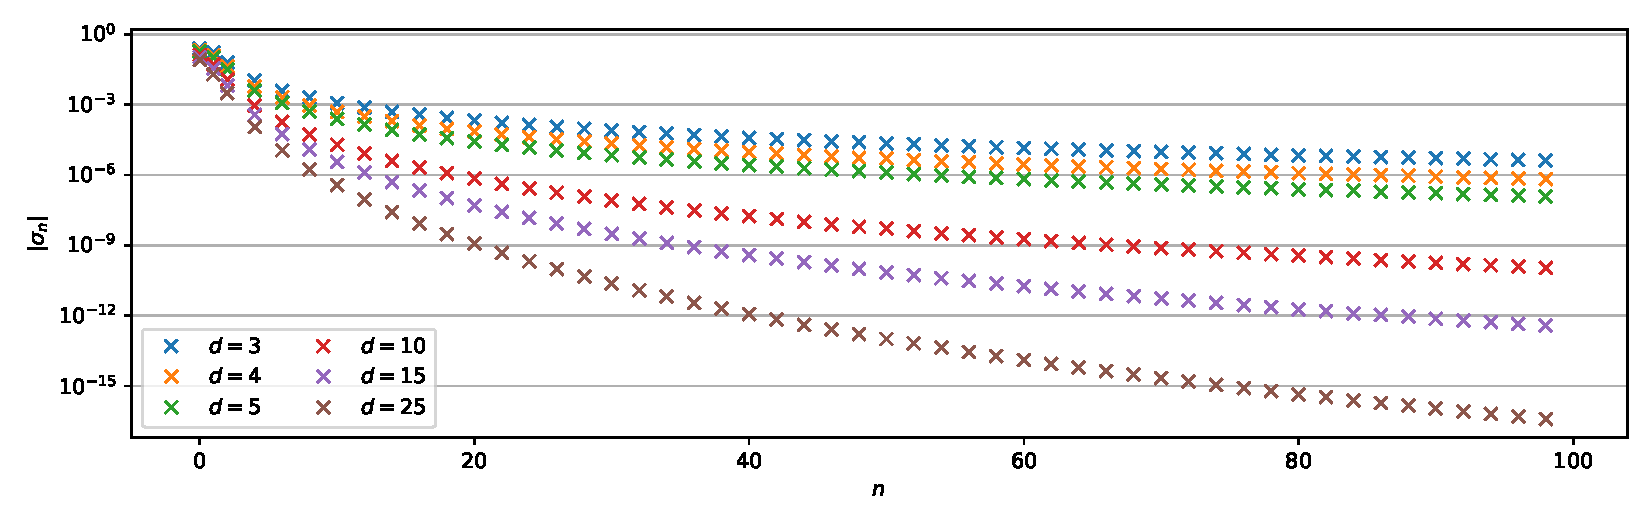
\includegraphics[width=\linewidth]{Appendix2/coefficients_relu.pdf}
    \caption{ReLU coefficients $\sigma_n$ as a function of degree $n$ for different dimensions $d$.}
    \label{fig:relu-coef}
\end{figure}

% \begin{figure}[t]
%     \centering
%     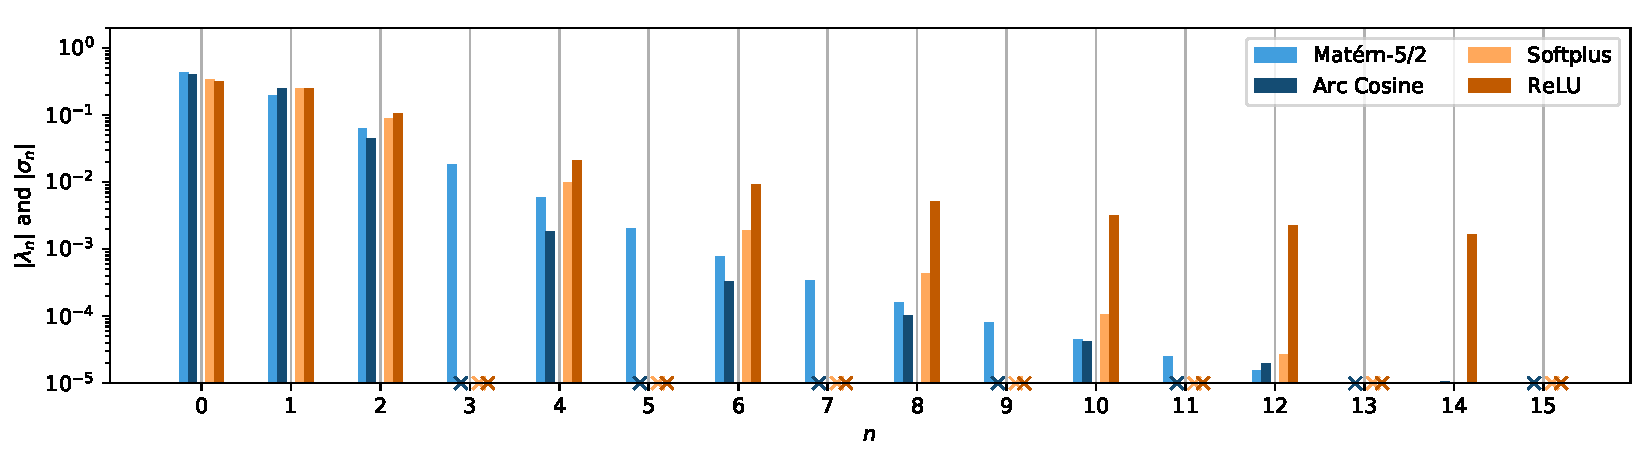
\includegraphics[width=\linewidth]{figures/spectra_kernels_and_activations.pdf}
%     \caption{Spectra of Arc Cosine and Mat\'ern-5/2 (blue), and ReLU and Softplus (orange) for different levels.}
%     \label{fig:spectra}
% \end{figure}